\chapter{Design del software} % Main chapter title

I diagrammi qui descritti sono quelli che effettivamente rappresentano il sistema sviluppato. 
Per una maggiore leggibilità, si è scelto di suddividere i diagrammi in base al sottosistema 
di appartenenza. \\
\indent I diagrammi delle classi riportati afferiscono a un diverso livello di dettaglio: 
per la parte front-end si è scelto di dare maggiore importanza alle interazioni e ai flussi 
di comunicazione tra i diversi strati del sottosistema, evitando di fare un "dump" speculare di tutto il codice sorgente e privilegiando solo la struttura logica, la separazione delle responsabilità e il flusso delle dipendenze tra i diversi livelli. \\
\indent Per quanto riguarda il lato back-end, il relativo modello di dominio e la descrizione delle
scelte di design adottate saranno trattati 
nella sezione dedicata. 

\section{Front-end}

Qui di seguito è illustrato il \textit{modello di presentazione}, evidenziando la struttura gerarchica dei componenti grafici. \\
\indent La figura 
mostra la struttura che consente di costruire l’albero dei componenti grafici. 
Ogni vista (\texttt{View}) è composta da componenti (\texttt{Component}) e può 
aggiungerne di propri con il metodo \texttt{addComponent()}; a loro volta i 
componenti possono contenerne altri, secondo la composizione ricorsiva. 
Le schermate (\texttt{Login} e \texttt{Dock}) specializzano \texttt{View}, 
mentre barre specializzano \texttt{Component}. Quali componenti contenga 
ciascuna schermata dipende dalla sua implementazione: per esempio \texttt{Regular} 
aggiunge l’\texttt{Assignmentbar} e \texttt{Administrator} la \texttt{Groupbar}. \\
\indent Il diagramma riporta i soli metodi che definiscono la composizione dei componenti, la 
navigazione tra componenti e tra schermate e le funzioni di base della finestra.
I metodi che riguardano la logica applicativa sono stati omessi, 
in quanto non contribuiscono a descrivere la struttura dell’albero. \\
\indent Nei successivi diagrammi, \guillemotleft use\guillemotright{} indicherà che
 un elemento ne impiega un altro (come tipo o come parametro);
  \guillemotleft call\guillemotright{} indicherà l'invocazione di un metodo statico e \guillemotleft create\guillemotright{} la creazione di
   un oggetto.

\newpage

\subsection{Strato \textit{View}}

\begin{figure}[!ht]
    \centering
    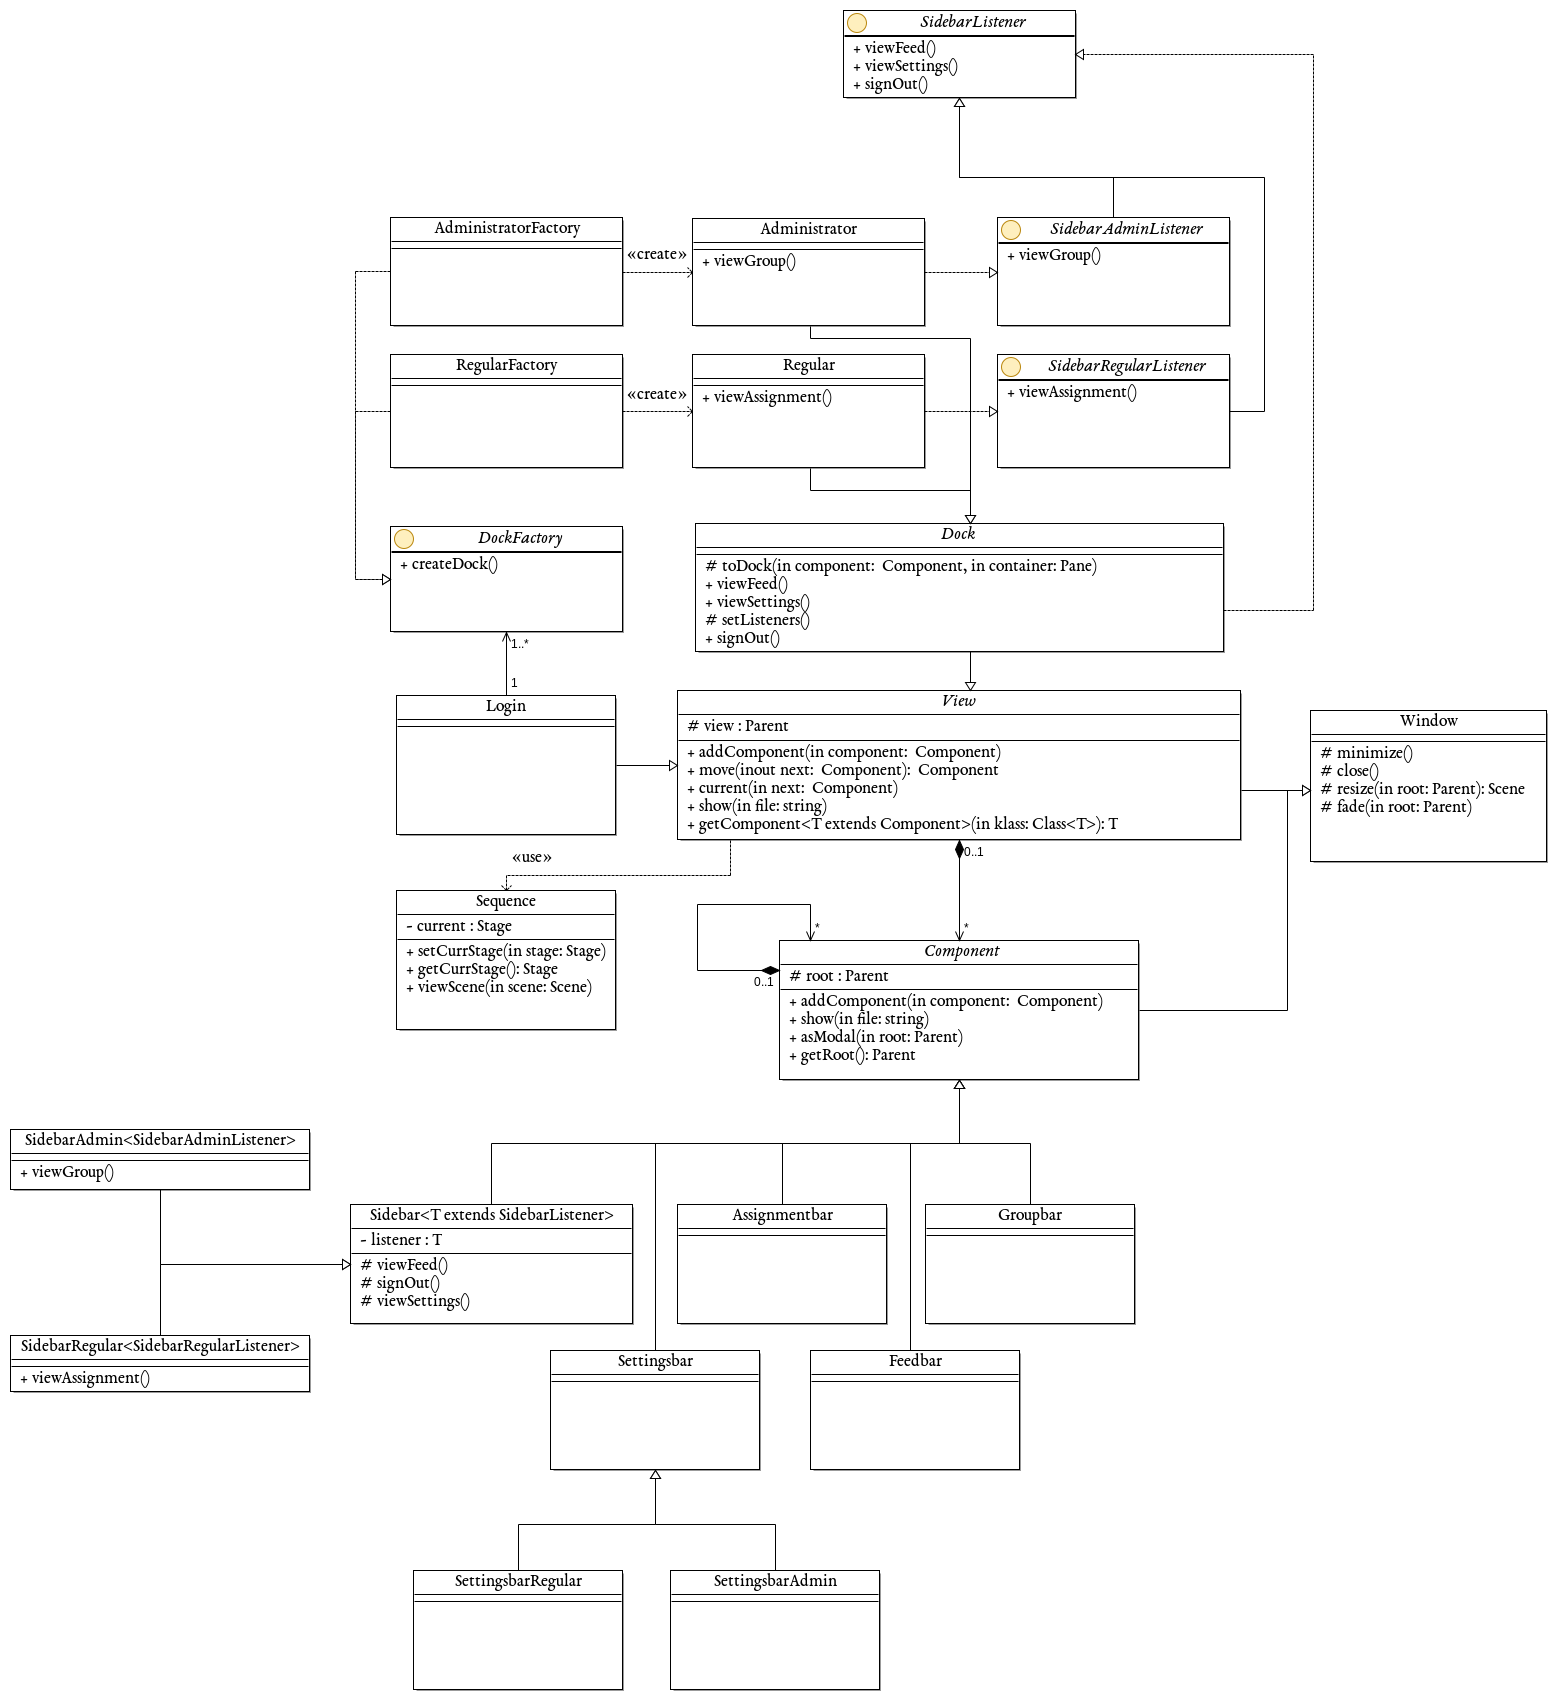
\includegraphics[width=15cm]{Chapters/Modello.png}
    \caption{Strato View}
    \label{fig:f1}
  \end{figure}

Il \texttt{Dock} è la schermata astratta che definisce la struttura 
comune alle schermate successive all'accesso; \texttt{Regular} e 
\texttt{Administrator} la specializzano aggiungendo i componenti propri 
del ruolo. \\
\indent Le classi \texttt{Feedbar}, \texttt{Groupbar}, \texttt{Sidebar}, \texttt{Assignmentbar} e \texttt{Settingsbar} sono componenti principali: contengono altri componenti, come le card e le modali rappresentate
nella figura 1.2, secondo
la composizione ricorsiva di \texttt{Component}. Sono loro a inserire nel proprio contenitore i
componenti che lo Strato \texttt{Presenter} restituisce già popolati con i dati provenienti dal
back-end. La struttura uniforme del pattern permette inoltre che uno stesso componente sia, a seconda del punto dell’albero in cui si trova, contenitore di altri componenti
oppure foglia. \\
\indent La schermata corretta è creata da una factory per ruolo, 
scelta da \texttt{Login} in base al ruolo restituito dal server. Le barre 
comunicano con la schermata che le ospita e vengono visualizzate tramite listener: \texttt{Sidebar} è
 parametrizzata sul tipo di listener, fissato dalle sottoclassi. La classe 
 \texttt{Window} raccoglie le funzioni di base della finestra e il 
 riferimento a \texttt{Orchestration}, mentre \texttt{Sequence} gestisce 
 la scena corrente. Le card e le finestre modali, 
 che specializzano \texttt{Component}, sono mostrate nella figura seguente.

\begin{figure}[!ht] 
\begin{center}
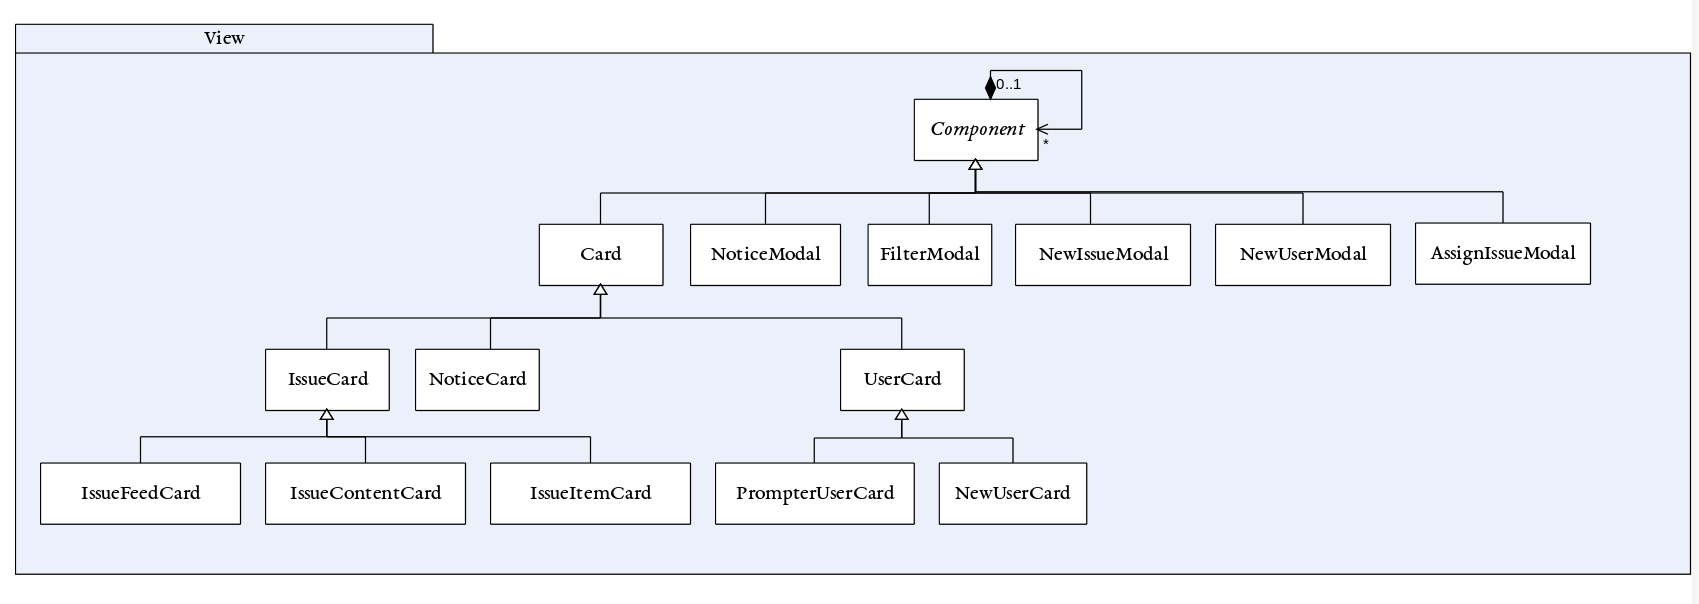
\includegraphics[width=\linewidth]{Chapters/composite.png}
\end{center}
\caption{Pattern gerarchico ricorsivo}
\label{fig:f1} 
\end{figure}

La struttura di questo pattern garantisce un'elevata estendibilità: qualora fosse necessario introdurre una nuova tipologia di componente grafico (es. la pagina della \texttt{Dashboard}), distinta da quelle già presenti nel sistema, è sufficiente definire una nuova classe concreta che estenda \textit{Component}. Grazie alla condivisione della classe astratta in comune, il componente grafico acquisisce immediatamente la capacità di inserirsi in qualsiasi punto della catena di composizione a runtime. \\
\indent Infine, è possibile arricchire  l'oggetto base con la nuova funzionalità senza dover modificare né la classe \textit{Component} e né i componenti preesistenti, aderendo rigorosamente al principio Open/Closed. \\
\indent Un altro vantaggio della composizione ricorsiva risiede nella gestione efficiente del ciclo di vita degli oggetti. Infatti, quando una vista viene rimossa, vengono rilasciati anche tutti i componenti che la compongono, semplificando enormente il lavoro da parte del Garbage Collector.

\indent È bene notare, che i componenti grafici sono stati 
rappresentati da classi spogliate sia dei metodi sia degli attributi. 
Il fine ultimo del diagramma è comunicare come il pattern
 organizzi i componenti grafici all'interno di un albero, il quale 
 riflette altresì la composizione gerarchica dei componenti descritti 
 dai file FXML.

Nella successiva figura si vedrà come sono organizzati 
gli orchestratori, che coordinano lo scambio di dati tra 
componenti e back-end.

\newpage

\subsection{Strato \textit{Presenter} (Orchestratori)}

 \begin{figure}[!ht] 
\begin{center}
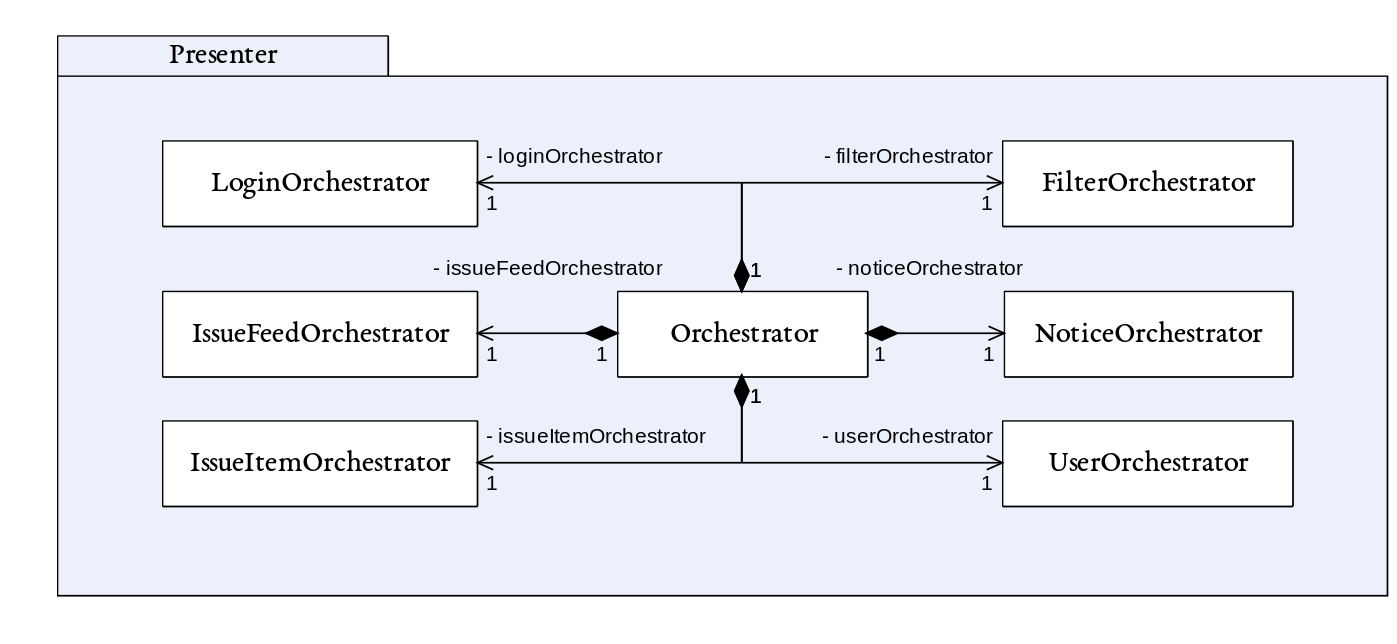
\includegraphics[width=13cm]{Chapters/composizione.png}
\end{center}
\caption{Proprietà dell'orchestratore}
\label{fig:f1} 
\end{figure}

La Figura 1.3 mostra la classe \texttt{Orchestrator}, che crea e possiede 
un’istanza di ciascun orchestrator concreto: la relazione 
è una composizione, perché gli orchestratori esistono finché 
esiste l’\texttt{Orchestrator}. L’applicazione ne crea una 
sola istanza, all’avvio, quindi ciascun orchestratore esiste 
in un solo esemplare, senza ricorrere a un Singleton né a 
metodi statici.

\subsubsection{Dalla \textit{View} al \textit{Presenter}: l’interfaccia \textit{IPresenter}}

\begin{figure}[!ht] 
\begin{center}
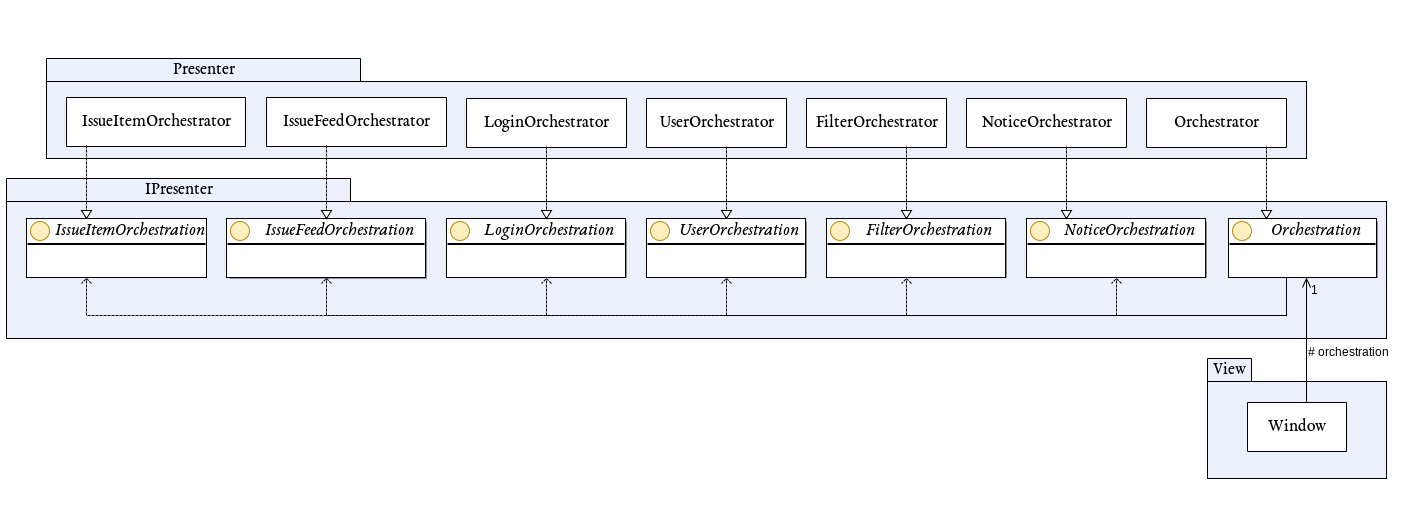
\includegraphics[width=15cm]{Chapters/presenter.png}
\end{center}
\caption{Strato View e Strato IPresenter}
\label{fig:f1} 
\end{figure}

La figura mostra il punto di contatto tra lo strato \texttt{Presenter} e le interfacce di \texttt{IPresenter}. La classe \texttt{Window}, radice della gerarchia di 
 \texttt{View} e di \texttt{Component}, custodisce un riferimento 
 all’interfaccia \texttt{Orchestration}, la cui implementazione è creata 
 una sola volta all’avvio. \\
\indent Il riferimento custodito da \texttt{Window} è uno stato globale: 
Tale scelta evita di propagare gli orchestratori lungo la catena dei 
costruttori che hanno come termine le viste e i componenti concreti. Inoltre, ogni classe appartenente 
alla gerarchia di \texttt{Window} è 
in grado di invocare l'orchestratore di cui ha bisogno, senza riferirsi agli oggetti
 dello strato \texttt{Presenter}. L'interfaccia \texttt{Orchestration} restituisce, per ciascuna funzionalità, 
il contratto corrispondente.

\subsubsection{Dal \textit{Presenter} alla \textit{View}: l’interfaccia \textit{IView}}

\begin{figure}[!ht] 
\begin{center}
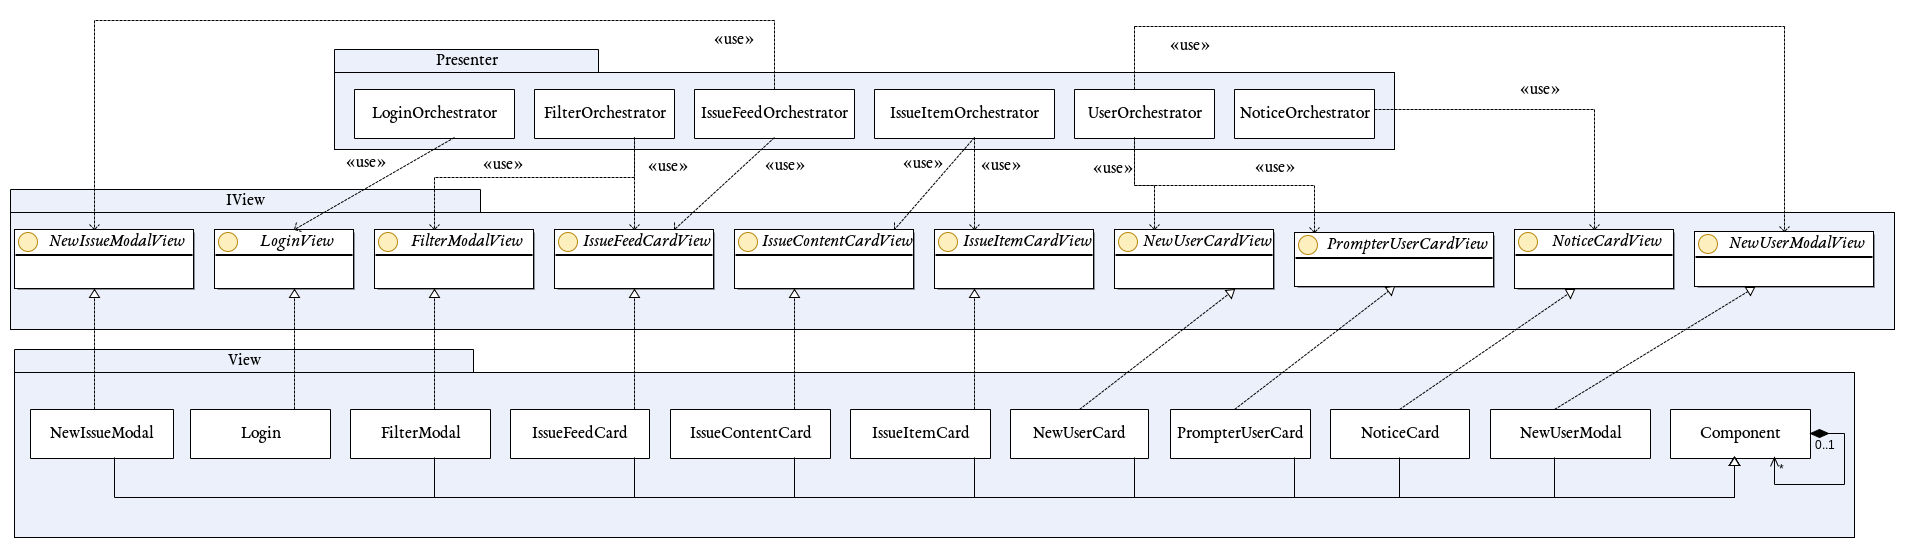
\includegraphics[width=\linewidth]{Chapters/IView.png}
\end{center}
\caption{Collegamento tra lo strato \texttt{Presenter}, le interfacce \texttt{IView} e lo strato \texttt{View}}
\label{fig:f1} 
\end{figure}

La Figura 1.5 mostra il verso opposto: il 
\texttt{Presenter} accede alle viste soltanto tramite le interfacce 
di \texttt{IView}, che le classi della \texttt{View} realizzano. Sono 
riportate le sole classi a cui il \texttt{Presenter} accede per scrivere 
o leggere i valori; classi come \texttt{Feedbar} e \texttt{Groupbar} 
non sono accedute dal \texttt{Presenter}, ma ne invocano i contratti tramite 
il riferimento a \texttt{Orchestration} presente in \texttt{Window}, 
come mostrato nella Figura 1.4.

Si prenda l'esempio della \texttt{NewIssueModal}, la finestra 
con cui si crea una nuova issue. Si supponga che l'utente
voglia creare una nuova issue. Il flusso di esecuzione
è il seguente.  L'utente compila i campi priorità, 
titolo, tipologia e così via all'interno della finestra  modale. 
La finestra invoca il 
metodo \texttt{create()} dell'orchestratore delle segnalazioni (\texttt{IssueFeedOrchestrator}) 
tramite il riferimento a \texttt{Orchestration}; l'orchestratore, tramite l'assembler,
 ne legge i valori con i metodi delle interfacce di vista \texttt{NewIssueModalView} eccezioni
 \texttt{IssueFeedCardView}, 
 costruisce l'oggetto per il back-end e lo invia. La risposta 
 viene convertita dal \texttt{mapper} in una \texttt{IssueFeedCard}, 
 che l'orchestratore restituisce alla \texttt{Feedbar} per la 
 visualizzazione. Assembler e mapper sono descritti nella 
 Figura 1.7.

\subsubsection{Dal \textit{Presenter} al \textit{Service}}

Lo strato \texttt{Presenter}, come specificato dal pattern, comunica con il back-end
mendiante lo strato \texttt{Service} che rispecchia i servizi forniti dalla parte
back-end. La seguente figura illustra chiaramente questa situazione.

\newpage

\begin{figure}[!ht] 
\begin{center}
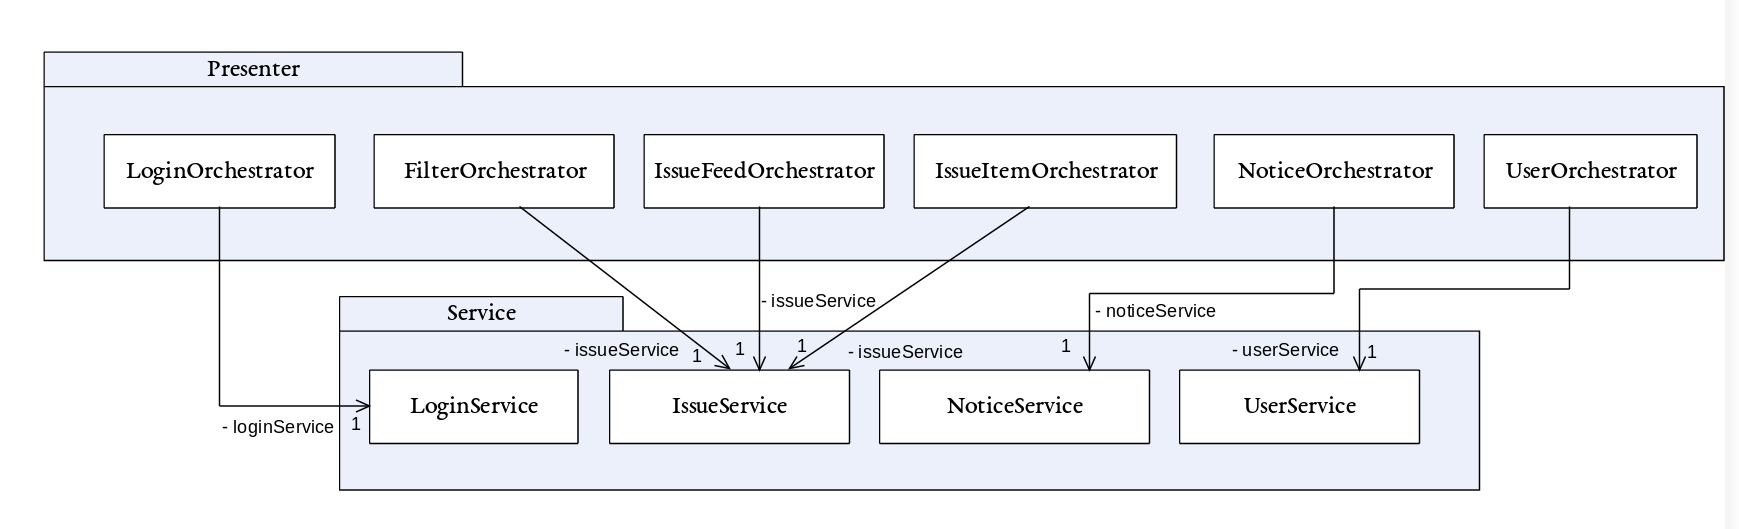
\includegraphics[width=\linewidth]{Chapters/presenter_service.png}
\end{center}
\caption{Collegamento tra lo strato \texttt{Presenter} e lo strato \texttt{Service}}
\label{fig:f1} 
\end{figure}

Questa figura mostra il 
collegamento tra lo strato \texttt{Presenter} e lo strato \texttt{Service}: 
ogni orchestratore possiede un riferimento al servizio della 
propria funzionalità. \\
\indent \texttt{FilterOrchestrator} e 
\texttt{IssueItemOrchestrator} usano \texttt{IssueService}, 
perché filtrare e consultare un elemento sono operazioni sulle 
segnalazioni. I servizi non conoscono gli orchestratori.

\subsubsection{Trasformazione dei dati: \textit{Assembler} e \textit{Mapper}}

\begin{figure}[!ht] 
\begin{center}
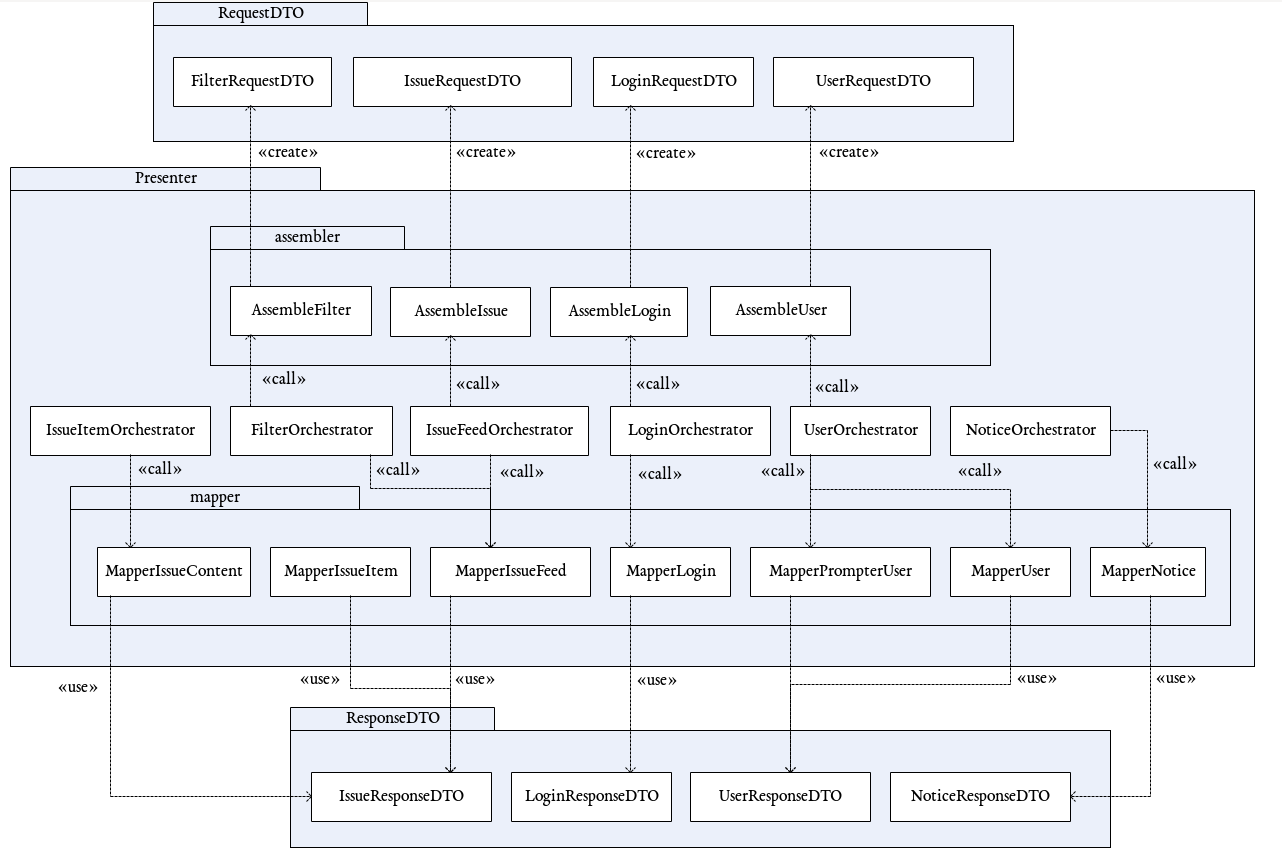
\includegraphics[width=\linewidth]{Chapters/assembler-mapper.png}
\end{center}
\caption{Collegamento tra lo strato \texttt{Presenter} e lo strato \texttt{Dto}}
\label{fig:f1} 
\end{figure}

La situazione rappresentata dalla Figura 1.7 descrive due momenti: il momento dell'impacchettamento 
dei dati per essere inviati al server, e il momento della conversione dei dati
ricevuti dal server stesso. \\
\indent Front-end e Back-end comunicano 
attraverso un contratto di comunicazione di informazioni, rappresentato 
dalle classi DTO. Gli orchestratori, tramite gli assembler, 
costruiscono a partire dai valori impostati nell’interfaccia le 
richieste in formato DTO. L'oggetto prodotto 
viene poi passato all'ultimo strato (\textit{Service}) che è il vero e 
proprio responsabile dell'invio dei dati.
I dati ricevuti dal server vengono successivamente convertiti nel 
componente grafico corretto. \\
\indent  Non tutte le funzionalità
hanno entrambi i collegamenti: le notifiche, ad esempio, solo in ricezione e
non richiedono un assembler. \\
\indent \texttt{FilterOrchestrator} usa 
\texttt{MapperIssueFeed}, perché i risultati di una ricerca sono segnalazioni.

\subsection{Strato \textit{Service}}

\begin{figure}[!ht] 
\begin{center}
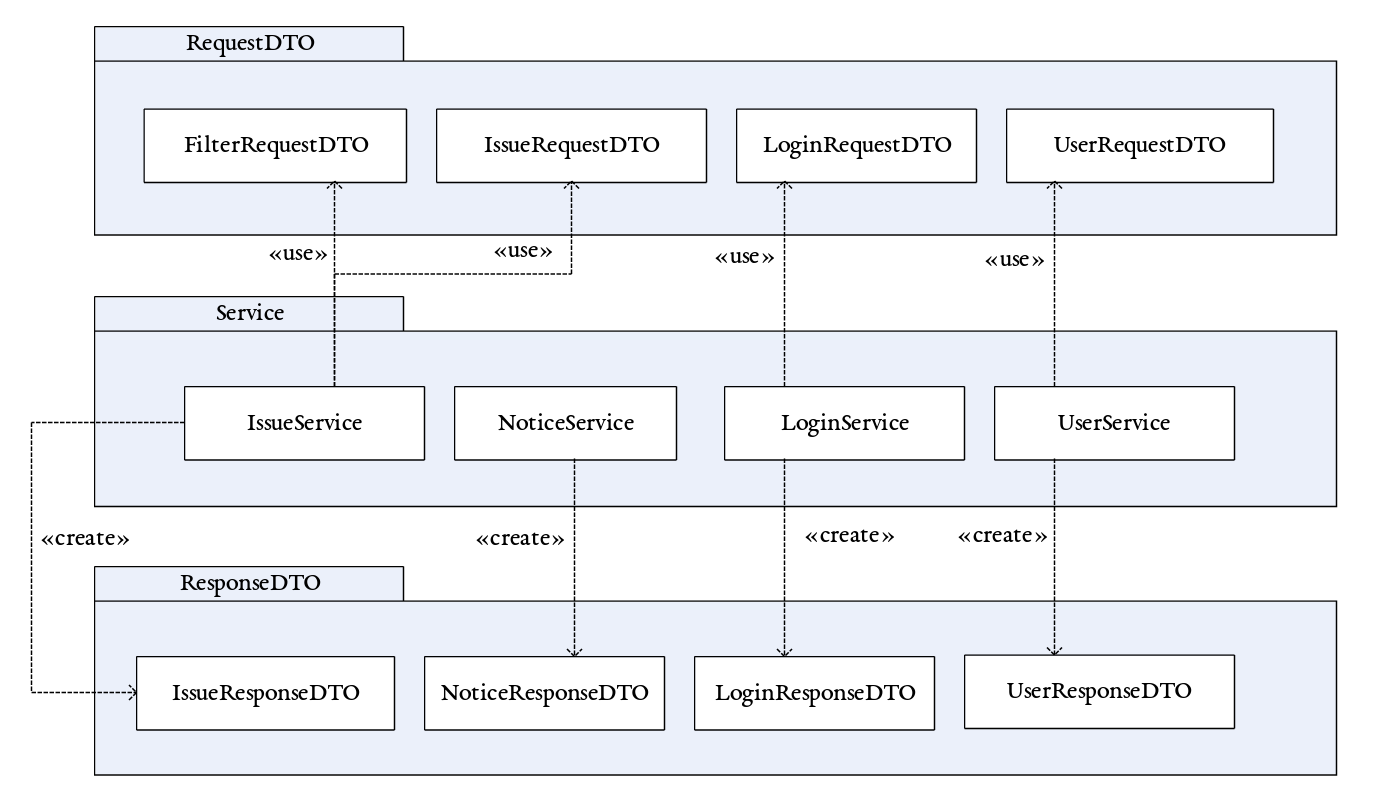
\includegraphics[width=15cm]{Chapters/service_dto.png}
\end{center}
\caption{Collegamento tra lo strato \texttt{Service} e lo strato \texttt{dto}}
\label{fig:f1} 
\end{figure}

Quest'ultima figura mostra l'ultimo punto di contatto dell'architettura. In tale situazione
le classi \texttt{Service} si servono dei contratti di comunicazione che definiscono il
formato di scambio dati con il back-end. Tali classi non conoscono 
il \texttt{Presenter} né la \texttt{View}: ricevono dall’orchestratore un oggetto di tipo
\texttt{RequestDTO}, con cui costruiscono la richiesta HTTP da inviare al server. \\
\indent La risposta del server viene convertita in un oggetto di tipo \texttt{ResponseDTO}, che il servizio restituisce 
all’orchestratore; come descritto nella Figura 1.7, questi lo passa al \texttt{mapper}, che lo converte nel 
componente grafico corretto. Le notifiche hanno 
solo la risposta, perché sono in ricezione. \\
\indent La dipendenza \textit{«use»} indica che le classi del package \texttt{Service} usano l’oggetto di tipo \texttt{RequestDTO} 
ricevuto come parametro. La creazione degli oggetti di tipo \texttt{ResponseDTO} è espressa invece dalla 
dipendenza \textit{«create»}.


\section{Back-end}
La presente sezione descrive le principali scelte fatte nel progettare
il codice del back-end e il motivo di ognuna di esse.
Qui di seguito è illustrato il \textit{modello di dominio}.

\begin{figure}[!ht] 
\begin{center}
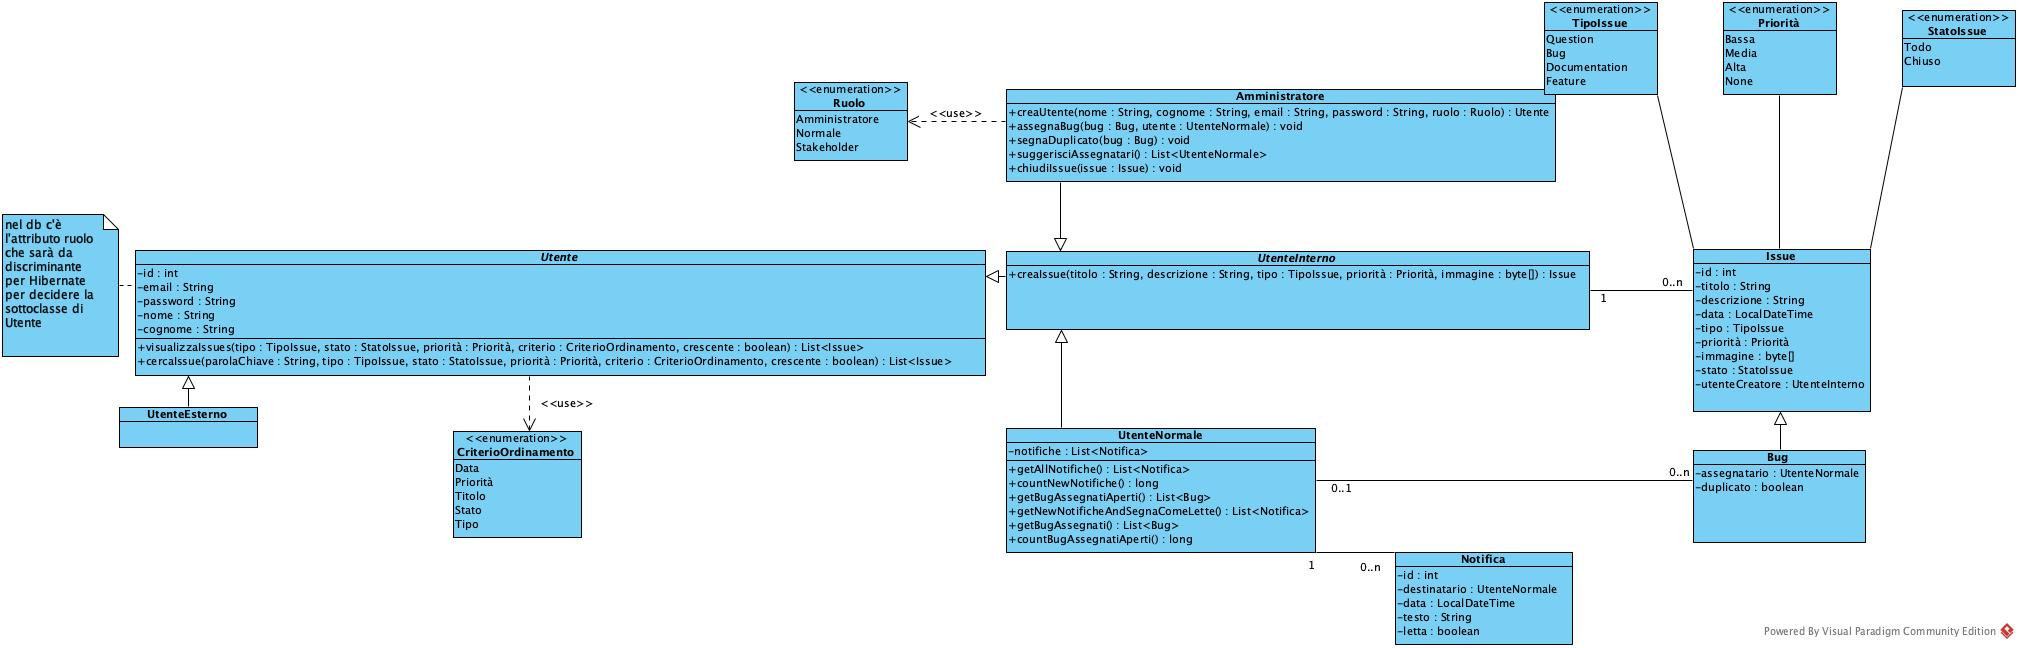
\includegraphics[width=\linewidth]{Chapters/modello di dominio.jpg}
\end{center}
\caption{Modello di dominio}
\label{fig:f1} 
\end{figure}

\subsection{I ruoli come sottoclassi}
I ruoli degli utenti non sono un campo da controllare con degli if, ma sottoclassi 
di Utente: Amministratore e UtenteNormale (entrambi UtenteInterno) e UtenteEsterno
 (lo stakeholder, che può solo consultare le issue). \\
 \indent In questo modo i permessi 
 diventano tipi: il creatore di un'issue è di tipo UtenteInterno, l'assegnatario di 
 un bug e il destinatario di una notifica sono di tipo UtenteNormale. È quindi il 
 compilatore a impedire, per esempio, che uno stakeholder risulti autore di un'issue, 
 senza controlli sparsi nel codice. 

 \subsection{Bug come sottoclasse di Issue }
 Solo i bug si possono assegnare e segnare come duplicati, quindi Bug è 
 una sottoclasse di Issue con i suoi campi in più (assegnatario e duplicato). \\
 \indent I metodi assegnaBug e segnaDuplicato ricevono un Bug: chiamarli su una question
  o una feature non è possibile. Il metodo creaIssue crea un Bug se e solo se 
  il tipo indicato è BUG. 

\subsection{Stato, priorità e duplicati }
 StatoIssue (TODO, CHIUSO) sta su Issue e non solo su Bug, perché 
 ogni issue nasce TODO e può essere chiusa. \\
\indent Priorita ha un valore NONE per "priorità non indicata" 
invece di null: così la priorità è sempre valorizzata, e filtrare o ordinare 
per priorità non richiede di gestire i valori mancanti. \\
\indent Il bug duplicato è indicato con un semplice valore vero/falso, senza un 
riferimento al bug originale: il requisito chiede solo di segnarlo e chiuderlo,
 e un riferimento in più avrebbe aggiunto vincoli senza una funzionalità che li usasse. 

\subsection{Organizzazione dei service}
I service sono divisi in due gruppi: 

Service "attore" (AmministratoreService, UtenteInternoService, UtenteNormaleService, UtenteService): contengono le operazioni del class diagram, 
cioè le azioni che un utente compie, raggruppate per la classe che le esegue. 

Service "di entità" (IssueService, BugService, NotificaService): contengono le operazioni 
di base e di supporto, che non sono azioni di un utente ma vengono usate dai service attore. 

La regola è: se un utente la compie come azione va nel service attore, se è un effetto 
di un'altra azione va nel service di entità. Per esempio creaNotifica sta in NotificaService 
e non in AmministratoreService, perché nessun utente "crea una notifica": la notifica è un 
effetto di assegnaBug, segnaDuplicato e chiudiIssue, che la riusano tutti. Così il codice 
segue il class diagram, e ogni service attore corrisponde a una sua classe. 

I service inoltre non controllano i permessi: non ricevono un parametro Amministratore 
per sapere chi li sta chiamando. I permessi si controllano prima, sugli endpoint (vedi 3c.4).
 L'utente loggato arriva al service solo quando è un dato dell'operazione, per esempio il 
 creatore di un'issue in creaIssue.

\subsection{DTO e validazione}
I controller non restituiscono mai le entità, ma dei DTO (Data Transfer Object): semplici 
record Java con i soli campi da mandare al client. Le entità non sono adatte a essere 
trasformate in JSON: 

 Utente contiene l'hash della password, che non deve uscire dal server. 

\noindent Alcune relazioni sono circolari (un utente ha le sue notifiche, ogni notifica 
ha il suo destinatario) e la conversione in JSON non finirebbe mai. 

Il JSON è il contratto con il front-end: con i DTO un cambiamento nel 
database non lo rompe. 

Anche i dati in ingresso arrivano come DTO (per esempio CreaIssueRequest) e 
vengono controllati su due livelli. I controlli di formato (campi obbligatori, 
lunghezze massime uguali a quelle delle colonne, formato dell'email, dimensione 
dell'immagine) sono annotazioni sui DTO, come @NotBlank e @Size, e rifiutano la 
richiesta prima che arrivi alla logica. Le regole di business (email già in uso, 
bug già chiuso, bug già duplicato) sono invece nei service.

\subsection{Sicurezza}
L'autenticazione usa Spring Security con la sessione HTTP: dopo il 
login il server ricorda l'utente e il client riceve un cookie da allegare 
alle richieste successive. All'inizio avevamo valutato i token JWT, ma li 
abbiamo scartati perché più complessi da gestire (firma, scadenza, rinnovo) 
senza vantaggi per un sistema con un solo back-end e un solo client. 
Le password sono salvate solo come hash BCrypt, e al login un'email 
inesistente e una password sbagliata danno lo stesso errore, per non 
rivelare quali email sono registrate. 

I permessi sono dichiarati con @PreAuthorize su ogni endpoint 
(per esempio hasRole('AMMINISTRATORE') per assegnare un bug): l'attore del 
class diagram diventa il ruolo richiesto dall'endpoint. Tutto tranne il login 
richiede di essere autenticati, quindi se ci si dimentica un'annotazione 
l'endpoint resta comunque chiuso a chi non ha fatto l'accesso. 

\subsection{Gestione degli errori}
I service segnalano i problemi lanciando eccezioni, e un'unica classe, 
GlobalExceptionHandler, le trasforma nella risposta HTTP giusta: 400 per dati non validi, 
401 per credenziali sbagliate, 404 per una risorsa inesistente, 409 per un'operazione in 
conflitto con lo stato attuale (per esempio assegnare un bug chiuso). Gli errori 401 e 
403 generati da Spring Security usano lo stesso formato. In questo modo i controller 
non hanno try/catch e il client riceve sempre errori con la stessa struttura, con un 
messaggio che può mostrare all'utente. 

\subsection{Regole di business}
Dove i requisiti lasciavano margine abbiamo deciso noi il comportamento: 

 creaUtente: l'email viene salvata in minuscolo e deve essere unica, 
per evitare due account con la stessa email scritta in modo diverso. 

 assegnaBug: un bug chiuso non si può assegnare. Se il bug passa 
da un utente a un altro, ricevono la notifica sia il nuovo sia il 
vecchio assegnatario. 

 suggerisciAssegnatari: gli utenti sono ordinati per numero di 
bug ancora aperti (TODO) assegnati, dal meno al più carico. 

 segnaDuplicato: un bug già segnato come duplicato non si può 
segnare di nuovo; il bug viene chiuso e l'assegnatario avvisato. 

 chiudiIssue: è riservata all'amministratore, e chiudere 
un'issue già chiusa non dà errore. 

\noindent Le operazioni che fanno più scritture insieme, come assegnaBug 
(aggiorna il bug e crea le notifiche), sono @Transactional: o riescono 
tutte o nessuna, così non restano notifiche di un'assegnazione mai avvenuta. 

\subsection{Filtri e ordinamenti nel database}
La vista delle issue permette di filtrare e ordinare per vari criteri. 
Invece di caricare tutte le issue e ordinarle in Java, abbiamo scritto 
le query in IssueRepository: una parte comune con i filtri e un ORDER BY 
diverso per ogni criterio e direzione. Il service sceglie la query giusta 
con uno switch. Così è il database, che lo fa in modo efficiente, a filtrare e 
ordinare, e al back-end arrivano solo le issue richieste. 

\section{Schema di persistenza dei dati}
In questa sezione descriviamo come Bugboard26 conserva i propri dati: 
quale database abbiamo scelto, come è fatto lo schema, come le classi del 
class diagram sono state trasformate in tabelle e come lo schema viene creato 
e aggiornato nel tempo. 

\subsection{Database e gestione dello schema}
Per la persistenza abbiamo usato MySQL 8, un database relazionale. I 
dati di Bugboard26 sono strutturati e collegati tra loro (un'issue ha un 
autore, un bug ha un assegnatario, una notifica ha un destinatario), quindi 
il modello relazionale, con le sue chiavi esterne e le transazioni, è quello più adatto. 

Lo schema è stato progettato con MySQL Workbench, disegnando prima il 
modello ER e generando poi automaticamente lo script SQL di creazione delle 
tabelle (forward engineering). 

Il back-end accede al database tramite JPA (con Hibernate come implementazione) e 
Spring Data JPA: le classi del dominio sono entità mappate sulle tabelle, e i 
repository offrono ai service le operazioni di lettura e scrittura. Hibernate 
però non crea le tabelle: è configurato in modalità validate, cioè all'avvio 
controlla soltanto che le entità Java corrispondano allo schema, e se non 
corrispondono l'applicazione non parte. Lo schema lo crea e lo aggiorna 
Flyway (vedi paragrafo 3.7). In questo modo è il database a comandare e il 
codice si adegua a lui, e non il contrario. 

\subsection{Schema ER}
Lo schema è composto da quattro tabelle: Utenti, Issues, Bugs e Notifiche. 

\begin{figure}[!ht] 
\begin{center}
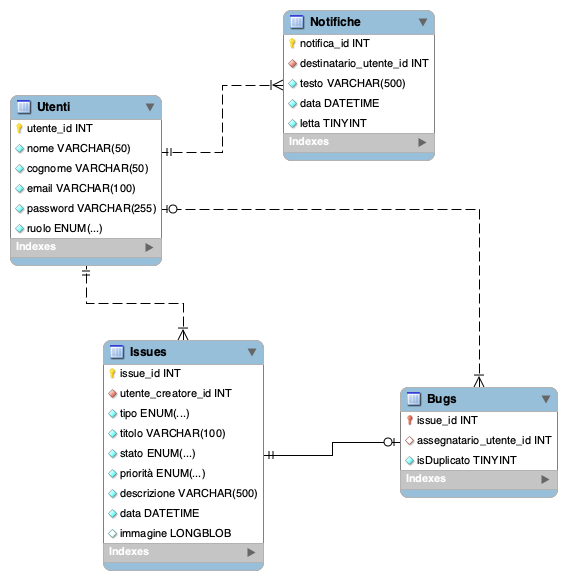
\includegraphics[width=10cm]{Chapters/schema ER.png}
\end{center}
\caption{Schema ER}
\label{fig:f1} 
\end{figure}

\newpage

La chiave gialla indica la chiave primaria, il rombo rosso una chiave esterna.
Il rombo pieno indica una colonna obbligatoria (NOT NULL), quello vuoto una 
colonna facoltativa. La linea tratteggiata indica una relazione non identificante, la linea 
continua una relazione identificante, in cui la chiave esterna 
ùfa parte della chiave primaria (è il caso di Bugs).

\section{ Report di qualità del codice}
Lo strumento utilizzato per assicurare un ottimo livello di qualità 
del codice del back-end è stato SonarQube for IDE, plugin per IntelliJ. 
Sono stati risolti tutti i warning e i code smells durante lo sviluppo del progetto, 
e per il report finale è stato usato SonaeQube Cloud: qui di seguito il summary 
indicante due errori relativi alla sicurezza, ma che sono in realtà scelte deliberate.

\begin{figure}[!ht] 
\begin{center}
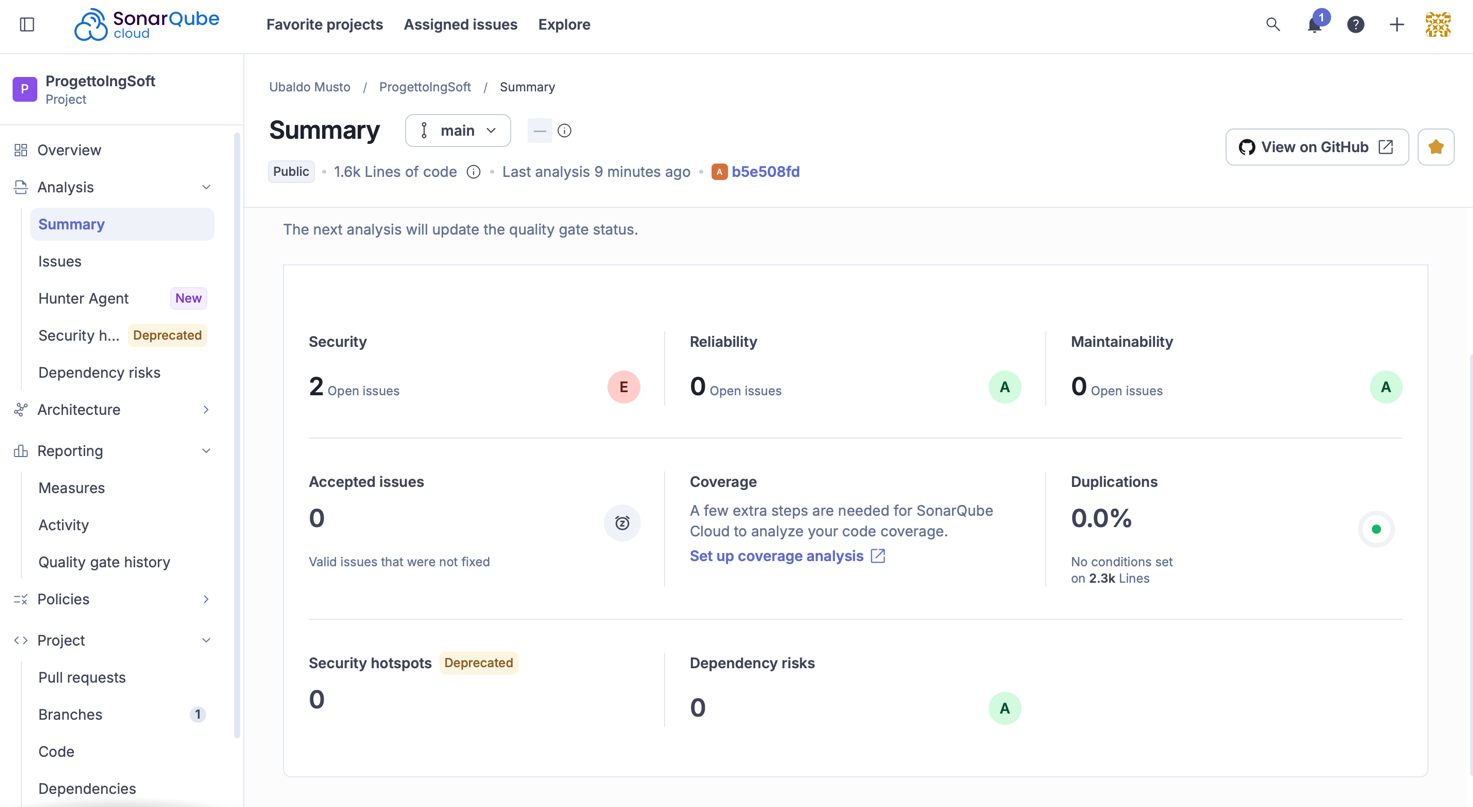
\includegraphics[width=\linewidth]{Chapters/report.png}
\end{center}
\caption{Report}
\label{fig:f1} 
\end{figure}

Data la natura del progetto si è optato di creare il primo utente admin direttamente 
dal codice, per ovviare a una moltitudine di problemi di testing e di demo su diverse
 macchine. Tale scelta però comporta la scrittura del nome utente ed ovviamente della 
 password (seppur sempre in formato hash) in maniera hardcoded, e ciò rappresenta una 
 falla di sicurezza.
Nel momento della messa in produzione del software una nuova migration Flyway risolve tutto.

\subsection{Protezione CSRF}
Questa problematica indica che la protezione CSRF (Cross-Site Request Forgery) di 
Spring Security è stata disattivata. Tale scelta è stata presa in quanto il CSRF è un 
attacco che sfrutta l'invio automatico dei cookie da parte del browser, ma il nostro
 client è un'applicazione JavaFX che gestisce da sé il cookie di sessione, quindi 
 l'attacco non è possibile e la protezione è stata disattivata.    
Se in futuro si aggiungesse un front-end web, la protezione andrebbe riattivata.   

\begin{figure}[!ht] 
\begin{center}
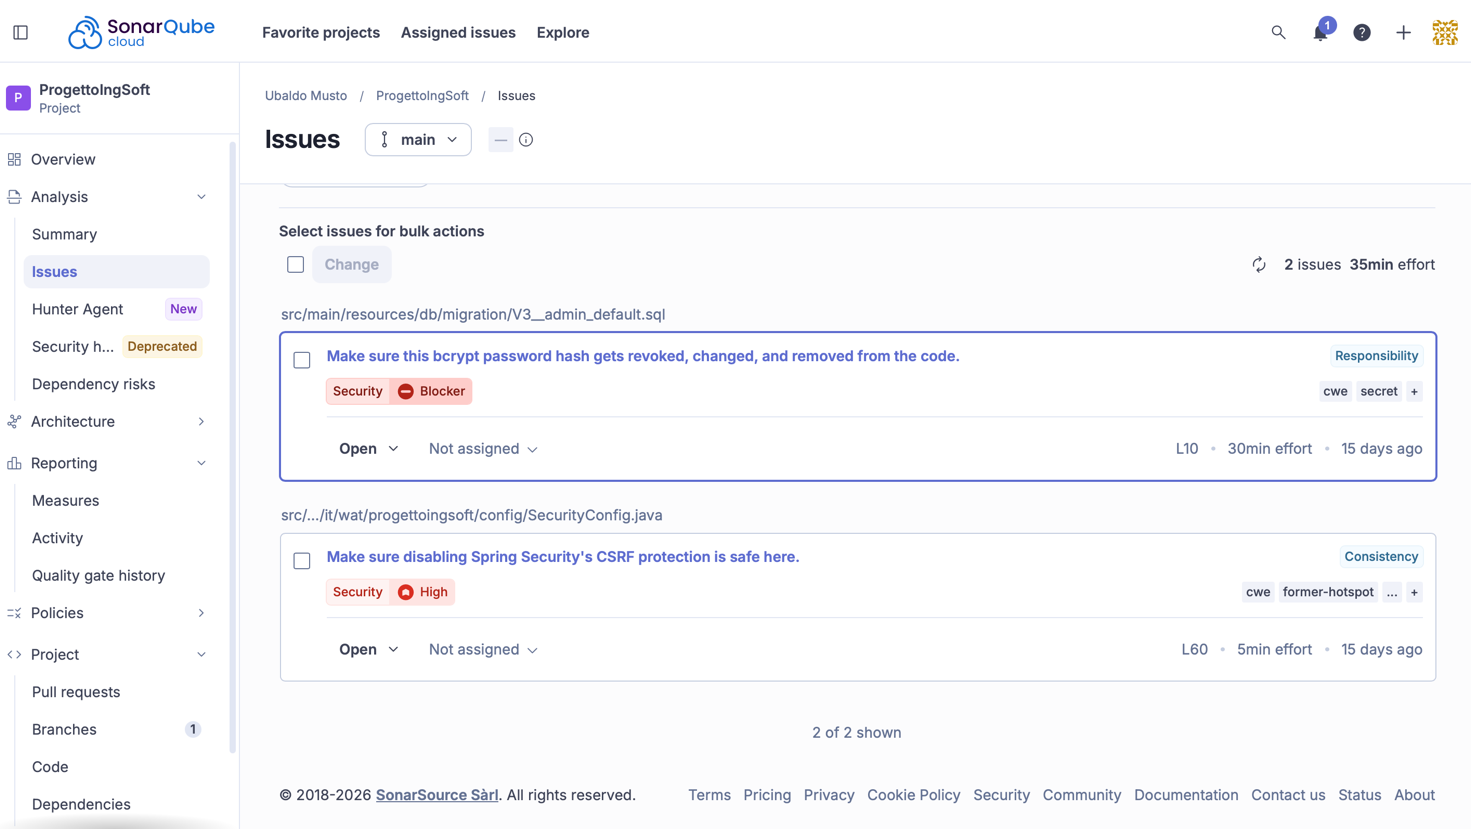
\includegraphics[width=\linewidth]{Chapters/report1.png}
\end{center}
\caption{Report}
\label{fig:f1} 
\end{figure}